\documentclass[authoryear,review,12pt]{elsarticle}

%\usepackage[utf8]{inputenc}
\usepackage{threeparttable}
\usepackage{subfig}
\usepackage{pdfpages}
\usepackage{amsfonts,amsthm,amssymb,amsmath}
\usepackage{graphicx,mathrsfs}
\usepackage{multirow}
\usepackage{float}
%\usepackage{tikz}
%\usetikzlibrary{arrows}
\usepackage[colorlinks,linkcolor=blue,citecolor=red]{hyperref}
\usepackage{natbib}
\usepackage{multicol}
%\bibliographystyle{chicago}
%
% page format
\usepackage[top=0.71in,bottom=0.781in,left=0.81in,right=0.81in%,a4paper
]{geometry}
\linespread{1.5}
\setlength{\parskip}{3.6pt}


%Natbib setup for author-year style

%\bibliographystyle{chicago}
\usepackage{float} 
\usepackage{multirow}
\newtheorem{algorithm}{Algorithm}
\newtheorem{theorem}{Theorem}
\newtheorem{definition}{Definition}
\newtheorem{lemma}{Lemma}
\newtheorem{example}{Example}
\newtheorem{remark}{Remark}
\newcommand{\rv}{random variable}
\newcommand{\bE}{\bf E}
\renewcommand{\Box}{\bigboxvoid}
\newcommand{\qeds}{$\qedsymbol $}
\newcommand{\R}{\mathbb{R}}
\newcommand{\Z}{\mathbb{Z}}
\newcommand{\cc}{\mathbb{c}}
\usepackage{ textcomp }
\usepackage{float} 
\usepackage{multirow}
\usepackage{comment}
%\usepackage{enumitem}
\usepackage{tikz}
\usepackage{algorithm}
\usepackage{adjustbox}
\usepackage{epstopdf}
\usetikzlibrary{arrows,decorations.pathreplacing,shapes}
\usepackage{amsmath}


\begin{document}

\title{Lagrangian Heuristic for Simultaneous Subsidization and Penalization:
\\[7pt]
 Implementations on Rooted Travelling Salesman Games}

\author[ustc]{Lindong Liu\corref{cor}}
\ead{ldliu@ustc.edu.cn}
\author[ustc]{Yuqian Zhou}
\ead{zyq94819@mail.ustc.edu.cn}
\author[ustc]{Zikang Li}
\ead{kk1996@mail.ustc.edu.cn}

\cortext[cor]{Corresponding author}

\address[ustc]{
\renewcommand{\baselinestretch}{1.5}
International Institute of Finance, School of Management,
\\[3pt]
 University of Science and Technology of China, Hefei 230026, China}

\begin{abstract}
This work examines the problem of stabilizing the grand coalition of an unbalanced cooperative game under the concept of  simultaneous subsidization and penalization (S\&P).
We design a generic framework for developing heuristic algorithms to evaluate the trade-off between subsidy and penalty in the S\&P instrument.
By incorporating some Lagrangian relaxation techniques, we develop an approach for computing feasible subsidy--penalty pairs under which the grand coalition is stabilized in unbalanced cooperative games.
This approach is particularly applicable when the characteristic functions of a cooperative game involve intractable integer programmes.
To illustrate the performance of the Lagrangian relaxation based approach, we investigate the rooted travelling salesman game, and the computational results obtained show that our new approach is both efficient and effective.\\
\end{abstract}

\begin{keyword}
Cooperative Game, Travelling Salesman Game, Cost Allocation
\end{keyword}

\maketitle
\date{\today}


\section{Introduction}\label{section:introduction}
Cooperative game theory investigates ways to enforce and sustain cooperation among a set of players; the key difficulty is in how to fairly allocate the costs (or profits) among different players by taking individual and group incentives into consideration (e.g., see \citealt{Jain2007CostSharing}).

Strictly, in terms of cost minimization, a cooperative game involving transferable utilities can be represented by a pair $(V,c)$, where $V = \{1,2,...,v\}$ denotes a set of players and $c:2^{|V|} \rightarrow \mathbb{R}$ is the characteristic function of the game. A subset of players, denoted by $s$, is called a coalition; while $V$ is the grand coalition, the set of all feasible coalitions is denoted by $S = 2^{|V|} \setminus \emptyset$. The characteristic function of the game is to specify for every coalition $s \in S$, a value $c(s)$, representing the minimum coalitional cost the members in $s$ have to pay in order to complete their work with cooperation.



To sustain cooperation in the grand coalition, the game requires a cost allocation vector $\theta= \big[\theta_1,\ldots,\theta_v\big]$, where $\theta_k$ is the cost assigned to player $k$ such that no individual or group of players has the incentive to deviate. By slightly modifying the notation for the sake of convenience, we use $\theta(s)=\sum_{k\in s}\theta_k$ to denote the total cost assigned to the players in coalition $s$.
Now, the grand coalition of the cooperative game $(V,c)$ will be stable, or the cooperative game $(V,c)$ will be balanced, if and only if the associating \textit{core} is non-empty (\citealt{bondareva1963some}), that is
\begin{eqnarray}\label{eqn:core}
\begin{aligned}
Core(V,c) = \bigg\{ \theta \in \R^v: \theta(V)=c(V) \mbox{ and } \theta(s) \leq c(s), \forall s \in S \setminus V \bigg\} \neq \emptyset,
\end{aligned}
\end{eqnarray}
where $\big\{ \theta(V)=c(V) \big\}$ is the budget balance constraint and $\big\{ \theta(s) \leq c(s),~ \forall s \in S \setminus V \big\}$ are the coalitional stability constraints (\citealt{shapley1969market}).

Due to the joint restrictions of the budget balance and coalitional stability constraints, the core of the cooperative game is sometimes empty.
In this case, to stabilize the grand coalitions in unbalanced cooperative games, researchers have developed several effective instruments, such as the instruments of subsidization, penalization, and simultaneous subsidization and penalization (S\&P).
The common idea of these instruments is to relax the concept of core (\citealt{curiel2013cooperative}).


In the instrument of subsidization, the central authority provides the grand coalition with a subsidy if they cooperate; the key problem is to find the minimum subsidy needed.
This instrument is closely related to the concept of \textit{$\gamma$-core} (\citealt{faigle1993some}) and the \textit{optimal cost allocation problem} (\citealt{Caprara2010LPB,LRCA2016}), where the central authority has to assign the players as much cost as possible such that the coalitional stability constraints in $(\ref{eqn:core})$ still hold.
Mathematically, the budget balance constraint in $(\ref{eqn:core})$ can be relaxed from $\big\{\theta(V) = c(V)\big\}$ to $\big\{\theta(V) \leq c(V)\big\}$, then we have
\begin{eqnarray*}\label{eqn:subsidy}
\begin{aligned}
\omega^* = \min_{\alpha} \bigg\{ c(V) - \alpha(V):~ \alpha(s) \leq c(s) \mbox{ for all } s \in S, ~\alpha \in \R^v \bigg\},
\end{aligned}
\end{eqnarray*}
where $\omega^*$ is the \textit{minimum subsidy} required for the grand coalition to cooperate and $\alpha(s)=\sum_{k\in s}\alpha_k$ for all $s \in S$.


As for the instrument of penalization, the central authority penalizes each sub-coalition for deviating from the grand coalition; hence, the problem is to minimize the penalty amount and reduce the players' dissatisfaction.
This instrument is similar to the concept of \textit{least core value} (\citealt{maschler1979geometric,schulz2010sharing}), where the cost assigned to each sub-coalition should not be more than the minimum coalitional cost plus the least core value, while the budget balance constraint in $(\ref{eqn:core})$ still holds.
Mathematically, the coalitional stability constraints in (\ref{eqn:core}) can be relaxed from $\big\{\theta(s) \leq c(s)\big\}$ to $\big\{\theta(s) \leq c(s)+z\big\}$ for all $s \in S \setminus V$, then we can formulate the penalization instrument as
\begin{eqnarray*}\label{eqn:lc}
\begin{aligned}
z^* = \min_{\beta,z} \bigg\{ z: ~\beta(V)=c(V), ~\beta(s) \leq c(s)+z \mbox{ for all } s \in S \setminus \{V\}, ~z \in \R, ~\beta \in \R^v \bigg\},
\end{aligned}
\end{eqnarray*}
where $z^*$ is the \textit{minimum penalty} required for the grand coalition to cooperate and $\beta(s)=\sum_{k\in s}\beta_k$ for all $s \in S$.

Recently, \cite{leastcore2018} introduced the new instrument of simultaneous subsidization and penalization (S\&P) by integrating the existing two instruments.
In the S\&P instrument, the central authority subsidizes the grand coalition if they cooperate, but at the same time penalizes each sub-coalition if they deviate.
For any given penalty $z$, the goal is to minimize the subsidy required to stabilize the grand coalition.
Mathematically, by relaxing both the budget balance and coalition stability constraints in (\ref{eqn:core}), the S\&P instrument solves
\begin{eqnarray}\label{eqn:SLC}
\begin{aligned}
z(\omega) = \min_{\beta,z} \bigg\{ z \in \R:\beta(V)=c(V)-\omega \mbox{ and } \beta(s) \leq c(s)+z,~\forall s \in S \setminus \{V\} \bigg\},
\end{aligned}
\end{eqnarray}
where $z(\omega)$ is the \textit{subsidized minimum penalty}.
In addition, as a function of subsidy $\omega$, $z(\omega)$ is also a subsidy--penalty function (SPF)\footnote{Note that \cite{leastcore2018} study the trade-off between subsidy and penalty in the format of penalty--subsidy function, i.e., PSF, $\omega(z)$.
Changing the format from PSF to SPF does not affect our future studies, but provides us with a perspective opposite to the S\&P instrument.
 \label{note1}}.


As an integration of subsidization and penalization, the S\&P instrument includes the two traditional instruments as its special cases.
To be specific, when subsidy is zero, the corresponding subsidized minimum penalty $z(0)$ will be equal to the least core value $z^*$, whereas when subsidy is $\omega^*$, the resulting minimum penalty $z(\omega^*)$ will be equal to zero. 
Therefore, following the S\&P idea and stabilizing the grand coalition in unbalanced cooperative games would be a good choice.


By broadly focusing on the integer minimization (IM) game, \cite{leastcore2018} developed the cutting plane (CP) and linear programming (LP) approaches based on the CP method and LP duality theory, respectively, to compute $\omega(z)$ for a given $z$.
The two approaches are effective under certain situations: the CP approach is effective when the corresponding separation problem is computationally tractable, and the LP approach is effective when the associating convex polyhedron is well identified.
However, computing the subsidized minimum penalty $z(\omega)$ for any given $\omega$ is in general hard due to the following reasons.
First, LP (\ref{eqn:SLC}) is a combinatorial optimization problem involving an exponential number of constraints.
Second, the characteristic function $c(s)$ is intractable in some IM games, such as machine scheduling (\citealt{leastcore2018}), facility location (\citealt{Kolen1983FL,Goemans2000FL,Puerto2011}), and travelling salesman (TSP) (\citealt{tamir1989core,kimms2016core}).


Following the concept of simultaneous S\&P, we develop a new heuristic algorithm based on the Lagrangian relaxation to compute the subsidized minimum penalty, $z^*(\omega)$, for an IM game.
We briefly summarize our major contributions to the literature as follows.

First, we design a new framework to develop heuristic algorithms for computing $z(\omega)$.
The key idea of the framework is to replace $c(s)$ for all $s \in S$ with its tractable bounds and reduce the computational difficulties for solving (\ref{eqn:SLC}).
Compared with the CP approach in \cite{leastcore2018}, this framework is efficient especially when $c(s)$ is computational intractable in some IM games.


Second, following the heuristic framework, we introduce the well-known Lagrangian bounds and develop an algorithm based on Lagrangian relaxation (LRB algorithm) for computing $z(\omega)$.
Compared with the LP approach in \cite{leastcore2018}, the LRB algorithm is effective since, for many integer linear programmings, Lagrangian bounds are sharper than linear relaxation bounds.
Furthermore, the LRB algorithm is able to deal with nonlinear situations while the LP approach is not.


Third, we implement our ideas in the rooted TSP games.
The result indicates the the effectiveness and efficiency of the LRB algorithm in computing $z(\omega)$, associating with a fair cost allocation. 
It also contributes to the TSP game's literature, which previously mainly focused on core existence checking and the time complexity analysis of the $\gamma$-core.


This paper is organized follows.
Section \ref{section:pre} formally introduces the concepts of simultaneous S\&P and IM games, and provides a TSP game example for illustration.
Section \ref{section:general} develops the LRB algorithm for computing the subsidized minimum penalty for IM games.
Section \ref{section:TSP} implements the LRB algorithm on the TSP game in order to demonstrate its effectiveness and efficiency.
Section \ref{section:conclusion} concludes the paper.


\section{Preliminaries}\label{section:pre}
There are some cooperative games in the field of operations research, such as facility location and machine scheduling games, whose characteristic functions are defined using intractable integer programmes.
These games can be included in the class of IM games studied in \cite{Caprara2010LPB}.
We once again define the IM game as follows for better illustration.

\renewcommand{\baselinestretch}{1.5}
\begin{definition}\label{defi:ORG}
A cooperative TU game $(V,c)$ is called an IM game if there exist\\
$~~\bullet$ positive integers $e$, $e'$, and $t$;\\
$~~\bullet$ left-hand side matrices $A \in \R^{e \times t}$ and $A' \in \R^{e' \times t}$;\\
$~~\bullet$ right-hand side matrices $B \in \R^{e \times v}$ and $B' \in \R^{e' \times v}$;\\
$~~\bullet$ non-negative right-hand side column vectors $D \in \R^{e}_+$ and $D' \in \R^{e'}_+$;\\
$~~\bullet$ an objective function $f(x)$ in $x$ \big($f(x)$ can be non-linear in this paper\big);\\
$~~\bullet$ an incidence vector $\gamma^s \in \{0,1\}^{v \times 1}$ with $\gamma_i^s=1$, where if $i \in s$, $\gamma_i^s=0$, otherwise, $\forall i \in V$,\\
such that the cost $c(s)$ equals the optimal value of the following integer programme for all $s \in S$:
\begin{equation}\label{eqn:orgc}
c(s) = \min_{x} \bigg\{ f(x):Ax \geq B\gamma^s + D, ~A'x \geq B'\gamma^s + D', ~x \in \{0,1\}^{t \times 1} \bigg\},
\end{equation}
where constraints in $(\ref{eqn:orgc})$ are divided into two parts for the usage of Lagrangian relaxation later in Section \ref{section:CGBAM}.
\end{definition}


It is known that many IM games are unbalanced, i.e., the associating grand coalition is unstable.
As described in Introduction, the S\&P instrument is proposed by \cite{leastcore2018} to stabilize the grand coalition, where an amount of subsidy, $\omega$, is provided to the grand coalition and an amount of penalty, $z(\omega)$, is imposed to the deviating sub-coalitions.
The key problem for the S\&P instrument is computing the subsidized minimum penalty $z(\omega)$ for any given subsidy $\omega$, where the resulting combinatorial optimization problem is
\begin{eqnarray*}
\begin{aligned}
z(\omega) = \min_{\beta,z} \bigg\{ z \in \R:\beta(V)=c(V)-\omega \mbox{ and } \beta(s) \leq c(s)+z,~\forall s \in S \setminus \{V\} \bigg\}.
\end{aligned}
\end{eqnarray*}
Below, we illustrate the S\&P instrument with a small example of a rooted TSP game as follows.
\renewcommand{\baselinestretch}{1.5}
\begin{example}\label{example:1}
Consider a rooted TSP game where node $1$ is the root, nodes $N_t=\big\{ 2,3,4,5,6 \big\}$ is a set of players, and $c(s)$ is the minimum transportation cost of the Hamiltonian cycle consisting of $s \cup \{ 1 \}$ for any coalition $s \subseteq N_t$. The network structure is given in Figure $\ref{figure:TSPExample}$, where the values on the arcs represent the corresponding transportation costs.
\end{example}
\begin{figure}[H]
\centering
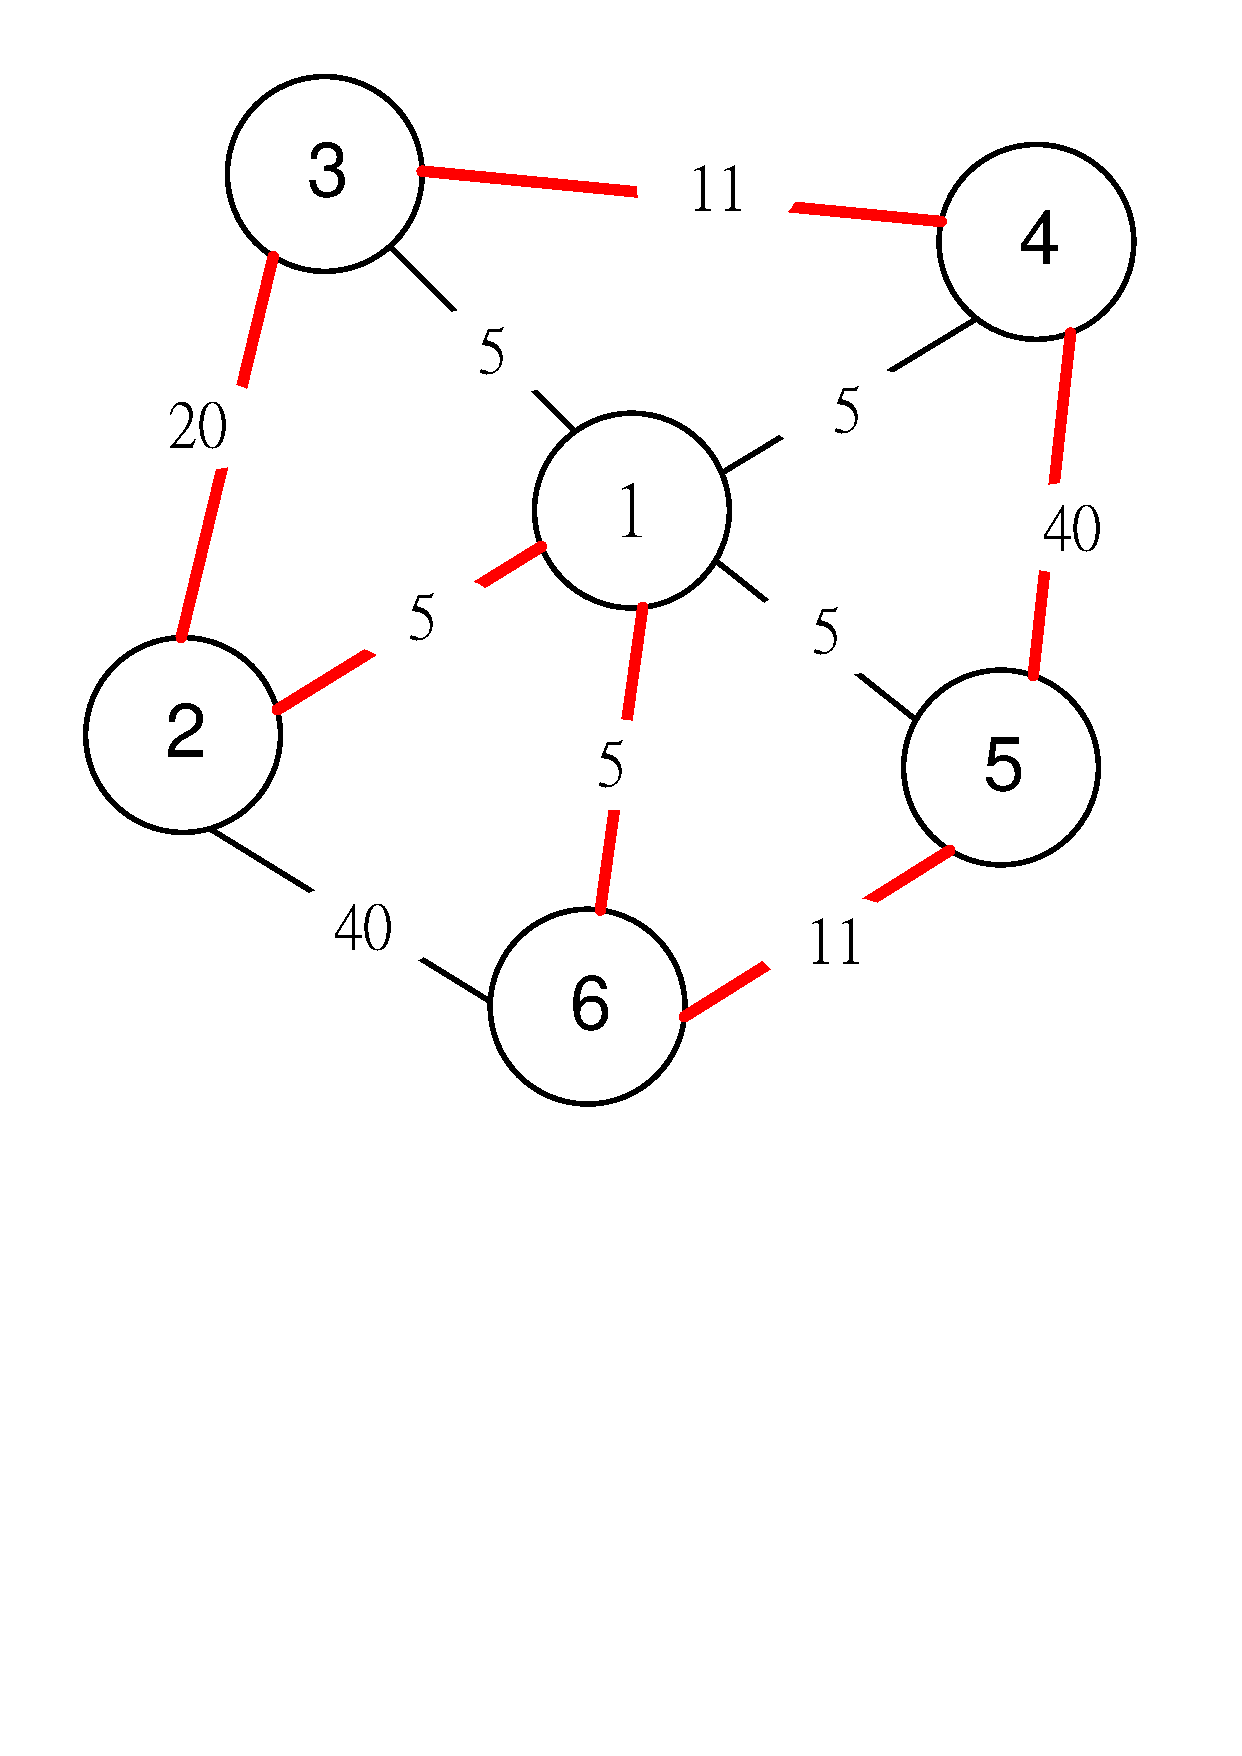
\includegraphics[width=0.3\textwidth]{ExampleTSP.pdf}
\caption{\label{figure:TSPExample}A rooted TSP game}
\vspace{-5mm}
\end{figure}

In Example \ref{example:1}, the grand coalition, representing the social optimum, has a minimum cost of $92$, with the optimal path being $1 \rightarrow 2 \rightarrow 3 \rightarrow 4 \rightarrow 5 \rightarrow 6 \rightarrow 1$.
By checking LP (\ref{eqn:core}), we can find that Example \ref{example:1} is unbalanced, that is, the core is empty.
Now, we stabilize the grand coalition by the S\&P instrument at different subsidy levels, and then compute the corresponding subsidized minimum penalty levels $z(\omega)$ with LP $(\ref{eqn:SLC})$. Some of the results are shown in Table~\ref{table:example1}.


\begin{table}[H]
\centering
\tabcolsep=16pt
%\small
\renewcommand\arraystretch{1.25}
\caption{\label{table:example1}subsidized minimum penalty for the rooted TSP game under different subsidy levels}
\vglue5pt
\begin{tabular}[!h]{c c c c c c c c c}
%\hline
%\multirow{1}{*}{} &\multicolumn{1}{c}{HG(\%)} &\multicolumn{1}{c}{TG(\%)}	&\multicolumn{1}{c}{$\bar{\omega}_{t}$(\%)}	&\multicolumn{1}{c}{$t_1$(s)}	&\multicolumn{1}{c}{$t_2$(s)}	&\multicolumn{1}{c}{$t_3$(s)}	&\multicolumn{1}{c}{Total time(s)}\\
\hline
$\omega$   &0	&6	&12	&18	&24	&30	&36	&42\\
\hline      
$z(\omega)$	&15	&12	&9.33	&7.33	&5.33	&3.33	&1.33	&0\\
$\beta(2,\omega)$	&25	&22	&19.33	&17.33	&15.33	&13.33	&11.33	&10                \\
$\beta(3,\omega)$	&20	&20	&19.33	&17.33	&15.33	&13.33	&11.33	&10                     \\
$\beta(4,\omega)$	&11	&11	&11	&11	&11	&11	&11	&10                     \\
$\beta(5,\omega)$	&25	&22	&19.33	&17.33	&15.33	&13.33	&11.33	&10                     \\
$\beta(6,\omega)$	&11	&11	&11	&11	&11	&11	&11	&10                     \\
\hline
\end{tabular}
\vspace{-2mm}
\end{table}

From Table \ref{table:example1}, we can see that, for example, if the subsidy provided by the central authority to the grand coalition is $\omega=6$, then the minimum penalty needed to be imposed to the deviating sub-coalitions is $z(\omega)=12$, and the resulting cost allocation vector is $\beta=[22,20,11,22,11]$.
According to \cite{leastcore2018}, as well as the results shown in Table \ref{table:example1}, the SPF $z(\omega)$ is decreasing, piecewise linear, and convex in $\omega$.
In addition, $z(0)$ is equal to the least core value, $z^*$, and $\omega^*$, such that $z(\omega^*) = 0$, is the minimum subsidy required to stabilize the grand coalition.

We can solve LP (\ref{eqn:SLC}) and derive all $z(\omega)$ and $\beta$ in Table \ref{table:example1} efficiently since there are only five players in the sample game.
However, when there are numerous number of players, it would be hard to optimally solve LP (\ref{eqn:SLC}) for the rooted TSP game due to its exponential number of constraints.
Note that, for each constraint in LP (\ref{eqn:SLC}), the computation of $c(s)$ is already hard in the TSP game (\citealt{woeginger2003exact}).


To apply the S\&P instrument to the IM game, \cite{leastcore2018} proposed two approaches (i.e., the CP and LP approaches) both of which can serve as approximation algorithms to solve LP $(\ref{eqn:SLC})$, i.e., $z(\omega)$, under certain conditions.
In the following section, we will develop an alternative approach to solve LP $(\ref{eqn:SLC})$, which outperforms the CP and the LP approaches from the perspective of efficiency and effectiveness, respectively.



\section{Design of Heuristic Algorithms}\label{section:general}
In this section, we first propose a generic framework to develop heuristic algorithms to solve LP (\ref{eqn:SLC}), assuming that we can obtain some upper and lower bounds for $c(s)$.
We then apply the well-known Lagrangian bounds to develop a practical approach for an approximate computation of the subsidized minimum penalty $z(\omega)$.


\subsection{A Generic Framework for Heuristic Algorithms}

For any $s \in S$, we denote $c_l(s)$ and $c_u(s)$, respectively, as the respective lower and upper bounds of $c(s)$. By respectively replacing $c(s)$ and $c(V)$ with $c_l(s)$ and $c_u(V)$, we can derive a restricted LP for $(\ref{eqn:SLC})$, expressed as
\begin{eqnarray}\label{eqn:aSLC}
\begin{aligned}
z_r(\omega) &= \min_{\beta,z}~ z\\
s.t.~~\beta(s) \leq c_l(s&)+z,~\forall s \in S \setminus \big\{V\big\},\\
\beta(V)=&c_u(V)-\omega.
\end{aligned}
\end{eqnarray}



\begin{theorem}\label{thm:rb}
The optimal value of LP $(\ref{eqn:aSLC})$ is the upper bound of the subsidized minimum penalty for an IM game $(V,c)$; that is $z_r(\omega) \geq z(\omega)$ for any given subsidy $\omega$.
\end{theorem}


As a penalty function shown in LP $(\ref{eqn:aSLC})$, $z_r(\omega)$ is referred to as the restricted subsidy-penalty function (R-SPF).
Since $z_r(\omega)$ is an upper bound of $z(\omega)$, the joint effect of penalty $z_r(\omega)$ and subsidy $\omega$ is that no coalition will deviate from the grand coalition $V$.


Similar to \cite{leastcore2018}, we can derive some properties of the R-SPF and evaluate the trade-off between subsidy $\omega$ and penalty $z_r(\omega)$ for stabilizing the grand coalition of IM game $(V,c)$.
The results are shown in Remark \ref{rem:convex}.

\begin{remark}\label{rem:convex}
Given any $c_u(V) \geq c(V)$ and $c_l(s) \leq c(s)$, $\forall s \in S$, for the R-SPF $z_r(\omega)$, we have,\\
(i) the R-SPF $z_r(\omega)$ is strictly decreasing, piecewise linear, and convex in subsidy $\omega$, and\\
(ii) for each linear segment of $z_r(\omega)$, its derivative $z'_r(\omega)$ is in the range $\big[ -\frac{v-1}{v}, -\frac{1}{v} \big] \subset \big[-1,0\big]$.
\end{remark}


Compared with LP $(\ref{eqn:SLC})$, we replace $c(s)$ with its tractable upper or lower bound. Thus, we might be able to solve LP $(\ref{eqn:aSLC})$ with some conventional combinatorial optimization techniques.
Theorem \ref{thm:rb} and Remark \ref{rem:convex} can be applied to any situation with different types of $c(s)$ bounds. 
In the following subsection, we develop a solution by applying Lagrangian bounds. 



\subsection{The Lagrangian Subsidized Minimum Penalty}\label{section:CGBAM}

Following Theorem~\ref{thm:rb}, we first need to obtain the Lagrangian lower bounds for $\big\{c(s):\forall s \in S\big\}$.
We can carry out a typical Lagrangian relaxation procedure by relaxing constraints $\{A'x \geq B'\gamma^s + D'\}$ in LP (\ref{eqn:orgc}) to the objective function with non-negative Lagrangian multipliers $\lambda$, and derive the Lagrangian characteristic function $c_{\lambda}(s)$ for an IM game $(V,c)$:
\begin{eqnarray}\label{eqn:lagrangianfunction}
\begin{aligned}
c_{\lambda}(s) = \min_{x} \bigg\{ f(x)-\lambda A'x + \lambda B'\gamma^s + \lambda D':Ax \geq B\gamma^s + D, x \in \{0,1\}^{t \times 1} \bigg\}, \forall s \in S.
\end{aligned}
\end{eqnarray}
In LP (\ref{eqn:lagrangianfunction}), $\lambda$ is a non-negative row vector with dimension $e'$, that is $\lambda \in \R_{+}^{1 \times e'}$. In particular, for the grand coalition $V$, the LP expression $(\ref{eqn:lagrangianfunction})$ is
\begin{eqnarray*}\label{eqn:lagrangianfunctionN}
\begin{aligned}
c_{\lambda}(V) = \min_{x} \bigg\{ f(x)-\lambda A'x + \lambda B'\textbf{1}+ \lambda D':Ax \geq B\textbf{1} + D, x \in \{0,1\}^{t \times 1} \bigg\}.
\end{aligned}
\end{eqnarray*}

As with usual Lagrangian relaxation, constraints $\{A'x \geq B'\gamma^s + D'\}$ can be chosen such that $c_{\lambda}(s)$ is relatively easy to solve, for example in (pseudo-)polynomial for any $s \in S$.

Since $c_{\lambda}(V)$ is a lower bound of $c(V)$ for any non-negative $\lambda$, to obtain the sharpest Lagrangian lower bound for $c(V)$, we need to solve the Lagrangian dual problem; that is we have to find the best Lagrangian multipliers $\lambda$ to maximize $c_{\lambda}(V)$: 
\begin{eqnarray*}\label{eqn:lagrangianfunctionmax}
\begin{aligned}
d(V) = \max_{\lambda} \bigg\{ \min_{x} \big\{ f(x)-\lambda A'x + \lambda B'\textbf{1} + \lambda D':Ax \geq B\textbf{1} + D, x \in \{0,1\}^{t \times 1} \big\}:\lambda \geq \textbf{0} \bigg\}.
\end{aligned}
\end{eqnarray*}

Then, the sub-gradient method (e.g., see \citealt{Ahuja1993NetworkBook}) can be applied to derive the optimal Lagrangian multipliers $\lambda^*$ for $d(V)$. The following discussion applies to any $\lambda$, not necessarily $\lambda^*$, although usually $\lambda^*$ leads to better results.



By substituting $c_l(s)$ with $c_{\lambda}(s)$ in LP $(\ref{eqn:aSLC})$, we can derive the associating Lagrangian subsidized minimum penalty problem as follows:
\begin{eqnarray}\label{eqn:laSLC}
\begin{aligned}
z_{\lambda}(\omega) = \min_{\beta,z} z~~&\\
s.t.~~ \beta(s) \leq  c_{\lambda}(s) + z,~ \forall s &\in S \setminus V,\\
-\beta(V) \leq -  c_u(V)+&\omega.
\end{aligned}
\end{eqnarray}

Note that by showing the second constraint in (\ref{eqn:laSLC}) as an inequality, we can simplify our future computations. This transformation is feasible because, as in Remark $\ref{rem:convex}$, $z_{\lambda}(\omega)$ is decreasing with respect to $\omega$.
From Theorem \ref{thm:rb}, %since $c_{\lambda}(s)$ is a lower bound on $c(s)$, we claim that 
the optimal $z_{\lambda}(\omega)$ to LP $(\ref{eqn:laSLC})$, or the Lagrangian subsidized minimum penalty, is an upper bound of the subsidized minimum penalty for the IM game $(V,c)$. 
In this case, given any subsidy $\omega$, the IM game $(V,c)$ can be balanced by letting the penalty deviate from the grand coalition to become $z_{\lambda}(\omega)$. % In addition, the corresponding Lagrangian $\omega$-subsidized least core cost allocation is given by optimal solution $\beta_{\lambda}(\ \cdot \ ,\omega)$. 


Motivated by \cite{LRCA2016}, the remainder of this subsection shows how to compute $z_{\lambda}(\omega)$ with Lagrangian decomposition and column generation techniques.


First, for any non-negative Lagrangian multipliers $\lambda$, we can decompose the Lagrangian characteristic function $c_{\lambda}$ into two sub-characteristic functions $c_{\lambda1}$ and $c_{\lambda2}$ such that $c_{\lambda}(s) = c_{\lambda1}(s) + c_{\lambda2}(s)$ under any $s \in S$, where
\begin{eqnarray*}\label{eqn:subcf1}
\begin{aligned}
c_{\lambda1}(s) = \lambda  B'\gamma^s,
\end{aligned}
\end{eqnarray*}
 and
 \begin{eqnarray*}\label{eqn:subcf2}
\begin{aligned}
c_{\lambda2}(s) = \min_x \bigg\{ f(x)-\lambda A'x  + \lambda D':Ax \geq B\gamma^s + D, x \in \{0,1\}^{t \times 1} \bigg\}.
\end{aligned}
\end{eqnarray*}

We define IM subgames 1 and 2 as $(V,c_{\lambda1})$ and $(V,c_{\lambda2})$, respectively. Note that the decomposition mode $(V,c_{\lambda1})$ is modular, that is $c_{\lambda1}(s_1)+c_{\lambda1}(s_2) = c_{\lambda1}(s_1 \cup s_2)$ for any two disjoint coalitions $s_1, s_2 \in S$. Now, we have an LP equivalent to $(\ref{eqn:laSLC})$, as shown in Lemma \ref{lemma:equivalentLP}.


\begin{lemma}\label{lemma:equivalentLP}
LP $(\ref{eqn:laSLC})$ has the same optimal objective function value as LP
\begin{eqnarray}\label{eqn:l2aSLC}
\begin{aligned}
z_{\lambda}(\omega) &= -\max_{\beta,z} -z\\
s.t. ~~ \beta(s) - z &\leq  c_{\lambda2}(s),~ \forall s \in S \setminus V,\\
 -\beta(V) \leq  -&c_u(V) + \omega  + c_{\lambda1}(V).
\end{aligned}
\end{eqnarray}
\end{lemma}


Next, we deal with the problems arising from the exponential number of constraints in $(\ref{eqn:l2aSLC})$.
By applying the column generation technique, we can solve $(\ref{eqn:l2aSLC})$ via its dual problem:
\begin{eqnarray}\label{eqn:master}
\begin{aligned}
\min_{\mu} \sum_{s \in S \setminus V} c_{\lambda2}(s&)\mu_s + \big[ \omega  + c_{\lambda1}(V) -c_u(V) \big]\mu_V,\\
s.t.~~\sum_{s \in S \setminus V}& \gamma_k^s \mu_s - \mu_V = 0,~\forall k \in V,\\
-&\sum_{s \in S \setminus V} \mu_s = -1,\\
&\mu_s \geq 0, ~\forall s \in S,
\end{aligned}
\end{eqnarray}
where $\{ \mu_s:\forall s \in S \} \in \R^{2^v-1}$ are the dual variables.
We summarize the procedures for solving the Lagrangian subsidized minimum penalty $z_{\lambda}(\omega)$ in Algorithm \ref{alg:SPC}.

\renewcommand{\baselinestretch}{1.5}
\begin{algorithm}[t]
\caption{LRB Algorithm to Compute $z_{\lambda}(\omega)$}
\label{alg:SPC}
\begin{description}
\item[Step 1.] For an IM game $(V,c)$, compute the Lagrangian bounds $c_{\lambda}(s)$ for $c(s)$, to obtain LP (\ref{eqn:laSLC}).

\item[Step 2.] Decompose $c_{\lambda}(s)$ into $c_{\lambda 1}(s)$ and $c_{\lambda 2}(s)$, and derive LP (\ref{eqn:l2aSLC}) and its dual LP $(\ref{eqn:master})$.

\item[Step 3.] Start from the restricted master problem of $(\ref{eqn:master})$, where the restricted coalition set is $S' \subset S$, with a polynomial number of elements, and compute its optimal dual solution $\pi^{*} \in \R^{v+1}$.
\item[Step 4.] Find a coalition $s^*$ with the minimum negative cost by solving the pricing problem,
\begin{eqnarray}\label{eqn:pricing}
\min_{s\in S\setminus S'} c_{\lambda2}(s) - \sum_{ k \in V} \gamma^s_k \pi_{k}^{*} + \pi_{v+1}^*.
\end{eqnarray}
\item[Step 5.] Following the duality theory, if there is a $\bar{s}$ with negative value of $(\ref{eqn:pricing})$, add the $\bar{s}$ into $S'$, and go back to step 3; otherwise (\ref{eqn:l2aSLC}) is optimally solved with its dual problem (\ref{eqn:master}), go to step 6.

\item[Step 6.] From the updated restricted coalition family $S'$ and its corresponding characteristic function values $\{c_{\lambda2}(s):\forall s \in S' \}$, the following LP gives the optimal Lagrangian subsidized minimum penalty:
\begin{eqnarray}\label{eqn:alpha2}
\begin{aligned}
z_{\lambda}(\omega) = &\min_{\beta,z} z\\
s.t.~~ \beta(s) - z \leq  c_{\lambda2}&(s),~ \forall s \in S' \setminus V,\\
-\beta(V) \leq  -c_u(V) &+ \omega  + c_{\lambda1}(V).
\end{aligned}
\end{eqnarray}
\vspace{-8mm}
\end{description}
\end{algorithm}


As we know, in column generation, when the pricing problem is hard to solve, one can take a compromised approach and find an $\bar s$ with a negative value of $(\ref{eqn:pricing})$, which will suffice till the last iteration.
However, this compromised approach is problem specific.
In Section \ref{section:TSP}, we show how to efficiently deal with the pricing problem in a rooted TSP game.
We refer to $z_{\lambda}(\omega)$, a function of $\omega$, as the Lagrangian R-SPF (LR-SPF).

\begin{lemma}\label{lemma:up}
By connecting a set of points $\bigg\{\big(\omega_0,z_{\lambda}(\omega_0)\big), \big(\omega_1,z_{\lambda}(\omega_1)\big), \ldots, \big(\omega_l,z_{\lambda}(\omega_l)\big)\bigg\}$ in the interval $\big[\omega_0,\omega_l\big]$, we can derive the upper bound $U_{\lambda}(\omega)$ on the curve of LR-SPF $z_{\lambda}(\omega)$ as well as SPF $z(\omega)$.
\end{lemma}

Lemma \ref{lemma:up} implies that the upper bound of the SPF curve $z(\omega)$ can be obtained by simply linking some discrete subsidy--penalty pairs $\big(\omega, z_{\lambda}(\omega)\big)$.
The accuracy of $U_{\lambda}(\omega)$ depends on both the accuracy of $z_{\lambda}(\omega)$ and number of points sampled.
From Remark \ref{rem:convex}, because the derivative of $z_{\lambda}(\omega)$ is within $\big[ -\frac{v-1}{v}, -\frac{1}{v} \big]$, the error between curves $U_{\lambda}(\omega)$ and $z_{\lambda}(\omega)$ is somehow bounded, but the error between $z_{\lambda}(\omega)$ and $z(\omega)$ for given $\omega$ still remains unknown.
Therefore, we need to find the lower bound of $z(\omega)$ in order to evaluate the effectiveness of the Lagrangian subsidized minimum penalty $z_{\lambda}(\omega)$.


\subsection{The Lower Bound of $z(\omega)$}\label{section:lowerbound}
We propose a method to calculate the lower bound $z_{k}(\omega)$, also called the $k$-level lower bound, of $z(\omega)$ by merely considering a subset of the constraints in LP~(\ref{eqn:SLC}). The value of $z_{k}(\omega)$ is obtained from LP,
\begin{eqnarray}\label{eqn:klevel}
\begin{aligned}
z_k(\omega) = \min_{\beta,z} &z\\
s.t.~~~\beta(s) \leq c_{u}(s)+z,~\forall s \in& S \setminus V \text{~and~} |s| \leq k,\\
\beta(s) \leq c_{u}(s)+z_,~\forall s \in S \setminus V& \text{~and~} |s| > v-k,\\
\beta(s) \leq c_{u}(s)+z_,~\forall& s \in S^{'\omega}_{\lambda},\\
\beta(V)=c_{\lambda}(V)&-\omega.
\end{aligned}
\end{eqnarray}

In LP $(\ref{eqn:klevel})$, $|s|$ represents the number of players in coalition $s$, and the coalition set $S^{\omega}_{\lambda}$ is a subset of the restricted coalition family $S'$ derived at the end of the LRB algorithm. For a given $k$, LP $(\ref{eqn:klevel})$ includes coalitions with no more than $k$ or no less than $v+1-k$ players, rendering the number of constraints in the order of $O(v^k)$.
To further tighten the lower bound, we add constraints $\big\{\beta(s) \leq c_{u}(s)+z_,~\forall s \in S^{'\omega}_{\lambda} \big\}$ to (\ref{eqn:klevel}), where $S^{'\omega}_{\lambda} = \big\{ s \in S': \beta_{\lambda}(s) - z_{\lambda}(\omega) =  c_{\lambda2}(s) \big\}$, since constraints $\big\{\beta(s) \leq c(s)+z_,~\forall s \in S^{'\omega}_{\lambda} \big\}$ are more likely to be tight when solving LP (\ref{eqn:SLC}).


\begin{lemma}\label{lemma:lower}
The optimal $z_k(\omega)$ derived from $(\ref{eqn:klevel})$ is the lower bound of the subsidized minimum penalty $z(\omega)$.
\end{lemma}

The lower bound given by LP $(\ref{eqn:klevel})$ is sharper when $k$ is larger, but when $k$ is no smaller than $\frac{v}{2}$, the corresponding lower bound $z_k(\omega)$ would be equal to $z(\omega)$, with the computation taking a very long time. For time efficiency, we compute only the two-level lower bound $z_2(\omega)$ in the rooted TSP game.



\section{Implementations on the Rooted TSP Game}\label{section:TSP}
In this section, we illustrate the LRB algorithm on the rooted TSP game, compute its Lagrangian subsidized minimum penalty, and investigate the quantitative relationship between subsidy and penalty in stabilizing its grand coalition.

\subsection{Game Definition}
The TSP game examined here is symmetric and rooted; that is the distances between two cities are the same in both directions, and there is a depot city. 
There is a complete undirected graph $G = (N_p \cup \{1\},E)$ with $N_p \cup \{1\}$ representing the city sites, $E$ being the set of edges linking these cities and city `1' being the depot city. Each edge $\{i,j\} \in E$ has a unit transportation cost of $c_{ji} = c_{ij} > 0$.
For a given coalition $s \in N_p$, the goal is to find a Hamiltonian circuit on cities $s \cup \{1\}$ with minimum total transportation cost. The notations used in the rooted TSP game are listed in Table~\ref{table:TSnotation}.
\begin{table}[H]
\tabcolsep=25pt
%\small
\renewcommand\arraystretch{1.25}
\caption{\label{table:TSnotation} Notations used in rooted TSP game}
\begin{tabular}[H]{c c}
\hline
\multicolumn{1}{c}{$N$} &\multicolumn{1}{l}{Set of city sites, $N=\left\{1,2,...,n\right\}$ with city $1$ being the depot.}\\
\multicolumn{1}{c}{$N_t$} &\multicolumn{1}{l}{Set of players, $N_t=\left\{2,3,...,n\right\}$.}\\
\multicolumn{1}{c}{$c_{ij}$} &\multicolumn{1}{l}{Cost to travel from city $i$ to city $j$, $\forall \{i,j\} \in N^2$.}\\
\multicolumn{1}{c}{$S$} &\multicolumn{1}{l}{Feasible player coalition set, $S = 2^{N_t} \setminus \emptyset$.}\\
\multicolumn{1}{c}{$s$} &\multicolumn{1}{l}{A feasible player coalition, $s \in S$.}\\
\multicolumn{1}{c}{$\gamma^s$} &\multicolumn{1}{l}{Incidence vector $\left[ \gamma^{s}_2,\gamma^{s}_3,...,\gamma^{s}_{n} \right]^T$, where $\gamma^{s}_j=1$, if $j \in s$, and $\gamma^{s}_j=0$, otherwise.}\\
\hline
\end{tabular}
\end{table}

\begin{definition}\label{defi:ug}
A rooted TSP game is defined as $(N_t,c_{t})$, with the player set $N_t$ and characteristic function $c_{t}(s)$ determined by integer linear program (ILP),
\begin{equation*}\label{eqn:tsobjective}
c_{t}(s) = \min_{x} \sum_{i \in N} \sum_{j \in N} c_{ij}x_{ij}
\end{equation*}
\begin{equation} \label{eqn:tscon1}
s.t.~~\sum_{i \in N}x_{ij} + \sum_{i \in N}x_{ji} = 2\gamma_j^{s\cup\{1\}}, ~\forall j \in N,
\end{equation}
\begin{equation}\label{eqn:tscon3}
\sum_{i \in \varphi} \sum_{j \in \varphi} x_{ij} \leq |\varphi| - 1, \forall \varphi \subset 2^{s \cup \{1\}} \setminus \emptyset,
\end{equation}
\begin{equation}\label{eqn:tscon2}
\sum_{i \in N} \sum_{j \in N} x_{ij} = |s|+1,
\end{equation}
\begin{equation}\label{eqn:tscon4}
x_{ij} \leq \frac{1}{2}(\gamma_i^{s\cup\{1\}}+\gamma_j^{s\cup\{1\}}),~\forall i \in N,~ j \in N,
\end{equation}
\begin{equation}\label{eqn:tscon5}
x_{ij} \in \{0,1\}, ~\forall i \in N, ~j \in N.
\end{equation}
\end{definition}

In the above ILP, constraints $(\ref{eqn:tscon1})$ are known as degree equations, which require the degree of a city to be `2' on the final trip if the city is in $s \cup \{1\}$; otherwise, the degree should be `0'. Constraints $(\ref{eqn:tscon3})$ are known as subtour elimination constraints ensuring that feasible tours should cover all cities in $s \cup \{1\}$. Constraints $(\ref{eqn:tscon2})$ and $(\ref{eqn:tscon4})$ are redundant due to $(\ref{eqn:tscon1})$, but they will be helpful in computing the Lagrangian lower bound and Lagrangian subsidized minimum penalty for the rooted TSP game.

In view of Definition~\ref{defi:ORG}, the rooted TSP game $ (N_t,c_{t})$ is an IM game $(V,c)$ with $V=N_t$ and $c = c_{t}$. The specific expressions of matrices $C$, $A$, $A'$, $B$, $B'$, $D$, and $D'$ can be obtained by transforming $c_{t}$ to a matrix format.



\subsection{Computation of the Lagrangian Subsidized Minimum Penalty}\label{section:LRBTSP}
In $c_{t}(s)$, by relaxing constraints $\big\{ \sum_{i \in N}x_{ij} + \sum_{i \in N}x_{ji} = 2\gamma_j^s: j \in N_t \big\}$ to the objective of Lagrangian multipliers $\sigma$, we can derive the Lagrangian characteristic function for the rooted TSP game as
\begin{eqnarray}\label{eqn:lrtscharacterristic}
\begin{aligned}
c_{\sigma}(s) = \min_{x} \sum_{i \in N} \sum_{j \in N} &\big(c_{ij} + \sigma_i + \sigma_j \big)x_{ij} - 2\sum_{j \in N_t} \sigma_j\gamma_j^s ~~~~(Let~\sigma_1 = 0) \\
&s.t.~~\sum_{i \in N}x_{i1} + \sum_{i \in N}x_{1i} = 2,\\
\sum_{i \in \varphi} &\sum_{j \in \varphi} x_{ij} \leq |\varphi| - 1, ~\forall \varphi \subset 2^{s \cup \{1\}} \setminus \emptyset,\\
&~~~~~~\sum_{i \in N} \sum_{j \in N} x_{ij} = |s|+1,\\
x_{ij} \leq \frac{1}{2}&(\gamma_i^{s\cup\{1\}}+\gamma_j^{s\cup\{1\}}),~\forall i \in N, ~j \in N,\\
&x_{ij} \in \{0,1\}, ~\forall i \in N, ~j \in N.
\end{aligned}
\end{eqnarray}

ILP $(\ref{eqn:lrtscharacterristic})$ shows that the redundant constraints $\big\{ \sum_{i \in N} \sum_{j \in N} x_{ij} = |s|+1 \big\}$ and $\big\{ x_{ij} \leq \frac{1}{2}(\gamma_i^{s\cup\{1\}}+\gamma_j^{s\cup\{1\}}):\forall i \in N, j \in N \big\}$ can improve the Lagrangian lower bound for $c(N_t)$. 
By dividing $c_{\sigma}$ into two parts, we can define the rooted TSP sub-games 1 and 2 as $(N_t,c_{\sigma1})$ and $(N_t,c_{\sigma2})$, respectively.

Sub-game 1 is modular, where the expression of $c_{\sigma1}(s)$ is
\begin{equation*}\label{eqn:tssub1}
c_{\sigma1}(s) = - 2\sum_{j \in N_t} \sigma_j\gamma_j^s,
\end{equation*}
and the specific expression of $c_{\sigma2}(s)$ is
\begin{eqnarray*}\label{eqn:tssub2}
\begin{aligned}
c_{\sigma2}(s) &= \min_{x} \sum_{i \in N} \sum_{j \in N} \big(c_{ij} + \sigma_i + \sigma_j \big)x_{ij},\\
&s.t.~~\sum_{i \in N}x_{i1} + \sum_{i \in N}x_{1i} = 2,\\
\sum_{i \in \varphi} &\sum_{j \in \varphi} x_{ij} \leq |\varphi| - 1, ~\forall \varphi \subset 2^{s \cup \{1\}} \setminus \emptyset,\\
&~~~~~~\sum_{i \in N} \sum_{j \in N} x_{ij} = |s|+1,\\
x_{ij} \leq \frac{1}{2}&(\gamma_i^{s\cup\{1\}}+\gamma_j^{s\cup\{1\}}),~\forall i \in N, j \in N,\\
&x_{ij} \in \{0,1\}, ~\forall i \in N, ~j \in N.
\end{aligned}
\end{eqnarray*}

In the literature, $c_{\sigma2}(N_t)$ is called a `1-tree problem' (e.g. \citealt{held1971traveling}). 
Similarly, we refer to $c_{\sigma2}(s)$ as a `1-s tree problem' with a subgraph $G=(N_t\cup\{1\},E)$ consisting of a tree on cities $s$ and two distinct edges at city 1 linked to $s$, and minimum transportation cost. 
To solve the 1-$s$ tree problem polynomially, we need to first construct a minimum spanning tree on cities $s$ and then add two edges linked to city 1 with the smallest transportation cost.

For ease of exposition, we rewrite $c_{\sigma2}(s)$ in an equivalent expression as
\begin{eqnarray*}\label{eqn:tssub2tree}
\begin{aligned}
c_{\sigma2}(s) = \min_{x} \sum_{i \in N} \sum_{j \in N} &c'_{ij}x_{ij}~~(c'_{ij} = c_{ij} + \sigma_i + \sigma_j)\\
s.t.~~&\text{$x$ is a 1-$s$ tree}.
\end{aligned}
\end{eqnarray*}

Now, we apply the LRB algorithm and compute the Lagrangian subsidized minimum penalty $z_{\sigma}(\omega)$ for the rooted TSP game. 
For this particular application of LRB algorithm, we omit all the detailed descriptions and analyse only its hardest part, the corresponding pricing problem. 
Specifically, this pricing problem can find the coalition $s \in N_t$ with the minimum negative cost:
\begin{eqnarray}\label{eqn:tspricinglcv}
\begin{aligned}
\min_{s \in N_t} \sum_{i \in N} &\sum_{j \in N} c'_{ij}x_{ij} - \sum_{j \in N_t} \gamma_j^s \pi_j^* + \pi_{n+1}^*\\
&s.t.~~\text{$x$ is a 1-$s$ tree},
\end{aligned}
\end{eqnarray}
where $\pi^*$ gives the optimal dual solution to the corresponding master problem defined in LP $(\ref{eqn:master})$. We denote the resulting Lagrangian subsidized minimum penalty for the rooted TSP game as $z_{\sigma}(\omega)$.


As stated in the description of Algorithm \ref{alg:SPC}, it is hard to optimally solve ILP $(\ref{eqn:tspricinglcv})$, but we can still apply the LRB algorithm before it is completed, because we only need to find column $\bar{s}$ with a minimum negative cost to continue the algorithm.


To further enhance computational efficiency, we adopt the Minimum Adjacency Test (see \citealt{duin1987some,ljubic2006algorithmic}) and reduce the magnitude of the problem $(\ref{eqn:tspricinglcv})$. 
This method is widely used to reduce the magnitude of prize-collecting Steiner tree problems. 
The key idea is to merge two cities into one if it does not affect the optimal value. With some modifications, we can obtain an efficient reduction technique for ILP $(\ref{eqn:tspricinglcv})$, as shown in Lemma \ref{lemma:reduction}. 
\begin{lemma}\label{lemma:reduction}
If the pricing problem $(\ref{eqn:tspricinglcv})$ has two nodes $a,b \in N_t$ such that
\begin{equation*}
\min \big\{ \pi_a^*, \pi_b^* \big\} - c'_{ab} >0 \text{~and~} c'_{ab} = \min_{ag \in N_t^2}c'_{ag},
\end{equation*}
then $a$ and $b$ can be merged into a new city $c$ with prize $\pi_c^* = \pi_a^* + \pi_b^* - c'_{ab}$ and transportation costs $c_{ic} = c_{ci} = min \{c_{ai}, c_{bi}\}$ for any $i \in N \setminus \{a,b\}$.
\end{lemma}

Although this does not guarantee polynomial time complexity, Lemma \ref{lemma:reduction} can greatly reduce the problem size when solving $(\ref{eqn:tspricinglcv})$ and ensure the time efficiency of the LRB algorithm when implementing a rooted TSP game. The computational results are shown in Section \ref{section:computationalresults}.



\subsection{Computational Results}\label{section:computationalresults}
In this subsection, we present our results of applying the LRB algorithm to the rooted TSP game.
We conduct experiments using a Windows 7 PC with an Intel Core i7-2600 running at 3.4GHz and 16G RAM. 
The algorithms are implemented with Matlab 2015a.

For our preliminary experiments, we first developed 50 TSP instances, each with 20 cities, including one root. 
The distances between two cities are uniformly distributed random values from 1 to 1000.
Note that further requiring triangle inequality in distance settings will not change our future computational procedures, but uniformly distributed distances can be used in some practical situations, such as for cases with weighted transportation costs.

For each instance, when computing the Lagrangian subsidized minimum penalty $z_{\sigma}(0)$ using Algorithm \ref{alg:SPC}, we found that 42 out of 50 instances are balanced; that is $z_{\sigma}(0) \leq 0$.
This result is not surprising, because when the transportation distance is uniformly distributed, players tend to visit less number of arcs, implying the preference of a single Hamiltonian circle including all the players; that is the grand coalition is stable.


To avoid trivial cases and consider more practical instances, we further clustered the cities from several regions whose distances from other cities in different regions are larger than those in the same region.
To be more specific, we divided the cities into groups and then multiplied the distances between two cities from different groups with random values ranging from 1 to 5.
Intuitively, it is hard to balance regional TSP cases because players from different regions are less willing to accept larger regional travelling costs.
The intuition is implied by our computational results where $z_{\sigma}(0) > 0$ for all the 50 regional TSP instances.
Note that regional situations are not rare in TSP problems.
For example, retailers always gather at the centre of different cities and request deliveries from a particular manufacturer.
In this case, the resulting TSP problem will be regional.


We conduct the following experiments with rooted and regional TSP instances, where the players are partitioned into 4, 5, 6, 7 and 8 regions, respectively, when there are 20, 25, 30, 35 and 40 cities.

First, for some visible examples, we give four representative Lagrangian SPF curves for TSP games in Figure \ref{figure:20partitioned}.
The curves are generated with the IPC algorithm proposed by \cite{leastcore2018}, and each subsidy--penalty pair on the curves is computed with Algorithm \ref{alg:SPC} (the LRB algorithm).


\begin{figure}[H]
\centering
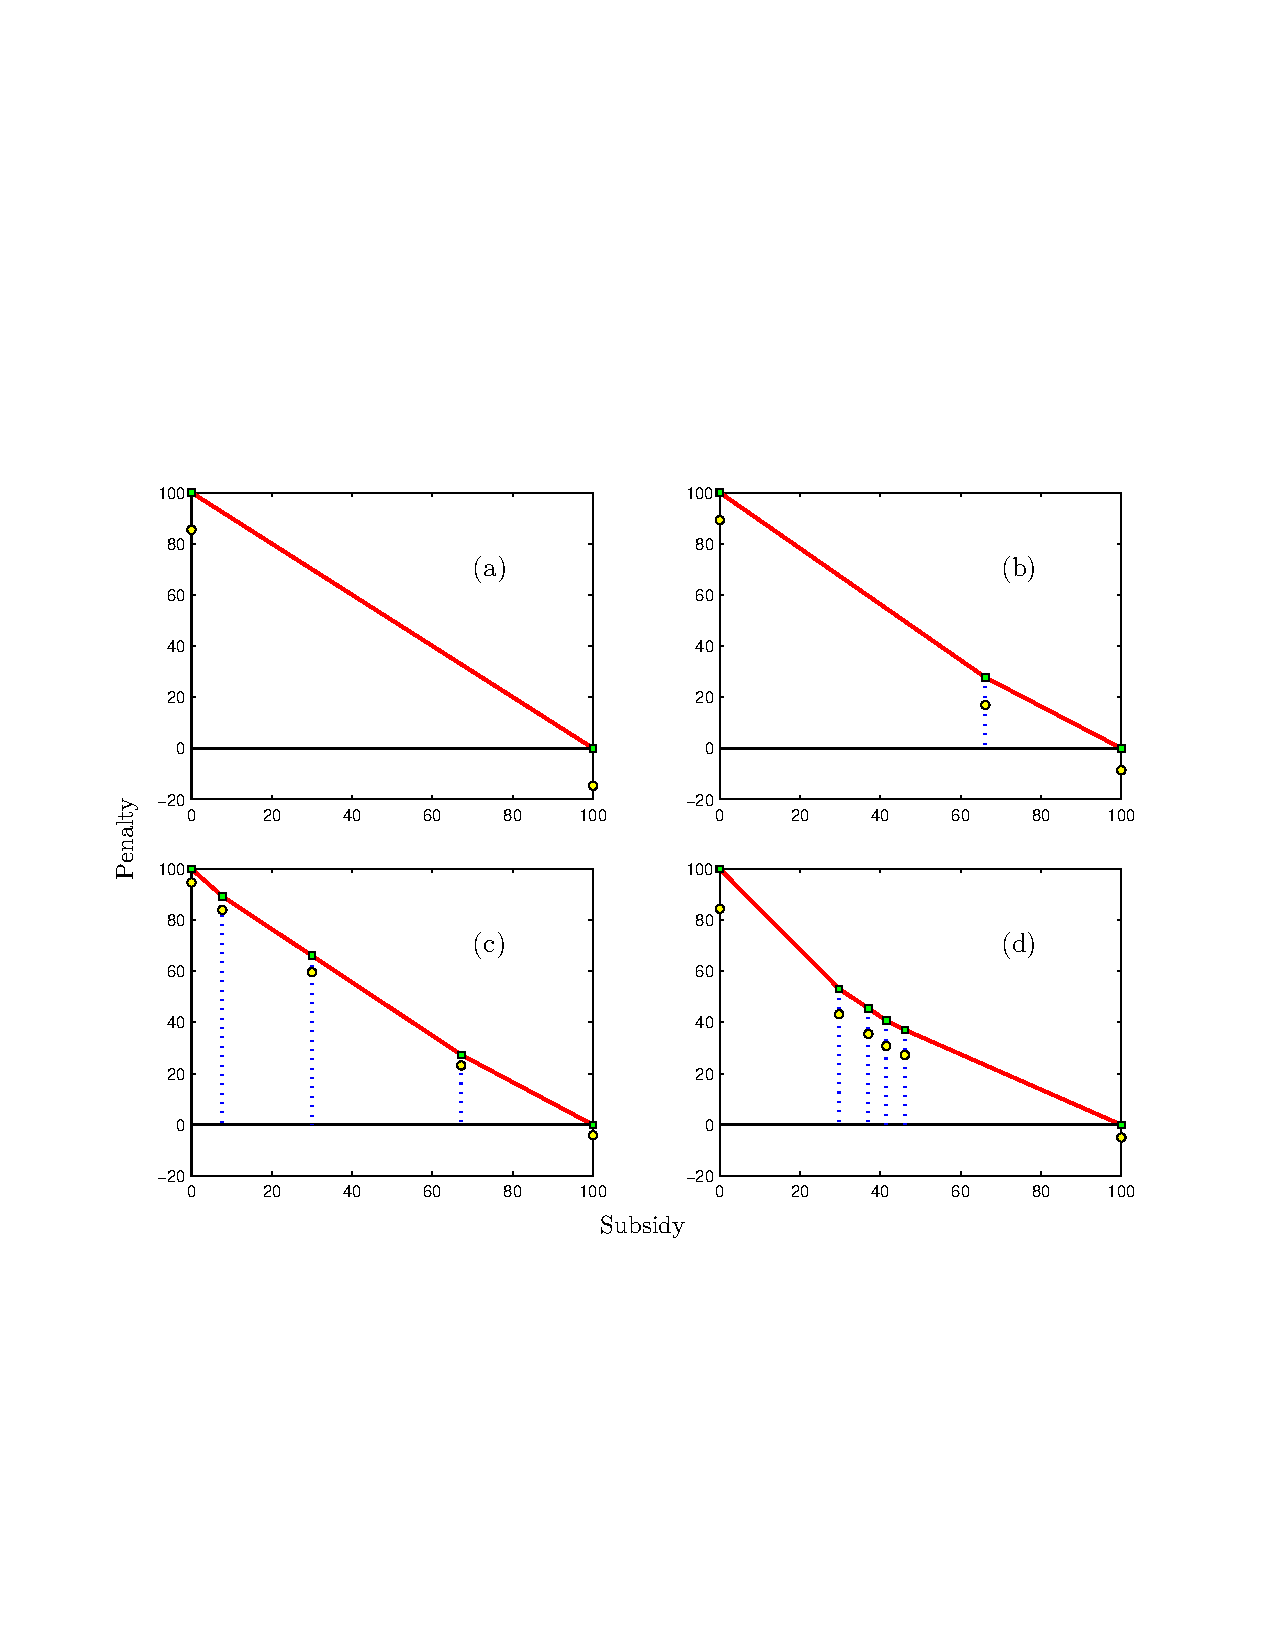
\includegraphics[width=1\textwidth]{e5.pdf}
%\captionsetup{font={small}}
\centering
\caption{\label{figure:20partitioned}Four representative Lagrangian SPFs for TSP games with 20 cities}
\end{figure}


In each diagram of Figure $\ref{figure:20partitioned}$, the curve represents the Lagrangian SPF $z_{\sigma}(\omega)$, and the dots below the curve represent the two-level lower bounds $z_{2}(\omega)$ at the corresponding subsidy levels.
For better understanding, all the subsidies and penalties are normalized in percentages of the corresponding Lagrangian minimum subsidy $\omega_{\sigma}$ and Lagrangian minimum penalty $z_{\sigma}(0)$, respectively.
Here, the Lagrangian minimum subsidy $\omega_{\sigma}$ is given by $\phi(N) - \alpha_{\sigma}(N_t)$, where $\phi(N)$ is the best social optimum (an upper bound) of the centralized TSP $c_t(N)$, and $\alpha_{\sigma}$ is the best cost allocation (a lower bound) of the optimal cost allocation problem $\alpha_t^*$.
Therefore, the Lagrangian minimum subsidy $\omega_{\sigma}$ is in fact the upper bound of the minimum subsidy $\omega_t^*$ for the TSP game.


From Figure $\ref{figure:20partitioned}$, the gap between $z_{\sigma}(\omega)$ $\big($upper bound of $z(\omega)$$\big)$ and $z_2(\omega)$ $\big($lower bound of $z(\omega)$$\big)$ is small.
To further show the effectiveness and efficiency of applying the LRB algorithm to TSP games, we present the average percentage gaps of $z_{\sigma}(\omega)$ against $z_2(\omega)$ and the average computational time of $z_{\sigma}(\omega)$ under different game sizes in Table \ref{table:detailed20}.


\begin{table}[H]
\centering
\tabcolsep=17pt
%\small
\renewcommand\arraystretch{1.0}
\caption{\label{table:detailed20}Computational results of the LBR algorithm’s effectiveness and efficiency}
\vglue5pt
\begin{tabular}[!h]{c c c c c c c c c}
\hline
\multirow{2}{*}{Size}  &\multicolumn{1}{c}{} &\multicolumn{3}{c}{Average Gaps (\%)}	&\multicolumn{1}{c}{} & \multicolumn{3}{c}{Time (in seconds)}\\
\cline{3-5}
\cline{7-9}
&	&Avg.	&Max	&Min	&	&Avg.	&Max	&Min\\
\hline
$n=20$	&	&6.57	&12.12	&2.54	&	&224	&468	&89\\

$n=25$	&	&6.32	&11.43	&3.06	&	&264	&879	&83\\

$n=30$	&	&6.39	&12.04	&2.13	&	&361	&960	&98\\

$n=35$	&	&6.21	&10.78	&2.78	&	&440	&1319	&122\\

$n=40$	&	&6.18	&11.41	&1.87	&	&564	&1552	&92\\
\hline
\end{tabular}
\end{table}
For each game size $n$ in Table \ref{table:detailed20}, we average the computational results over 50 randomized instances.
We find the LRB algorithm effective for computing Lagrangian subsidized minimum penalties for TSP games.
Compared to the two-level lower bounds $z_2(\omega)$, the average gap of $z_{\sigma}(\omega)$ is around 6.25\% with different game sizes.
We also observe an increasing tendency of performance of the LRB algorithm implemented on larger sizes of TSP games.
Note that the gap of $z_{\sigma}(\omega)$ could be further narrowed by comparing it with sharper lower bounds $z_k(\omega)~(k >2)$, or finding tighter $\phi(N)$ for the cost of grand coalition in the TSP game.


We now check the overall trade-off between the subsidy $\omega$ and penalty $z_{\sigma}(\omega)$ in Figure \ref{figure:differentsize} for TSP games.
We again average the results over 50 randomized instances for each game size.
For each game instance, we consider five different subsidy levels by setting $\omega$ at 0\%, 20\%, 40\%, 60\,% and 80\% of $\omega_{\sigma}$ respectively,
and the penalty levels are normalized in the percentage ratios against $z_{\sigma}(0)$.
\begin{figure}[H]
\centering
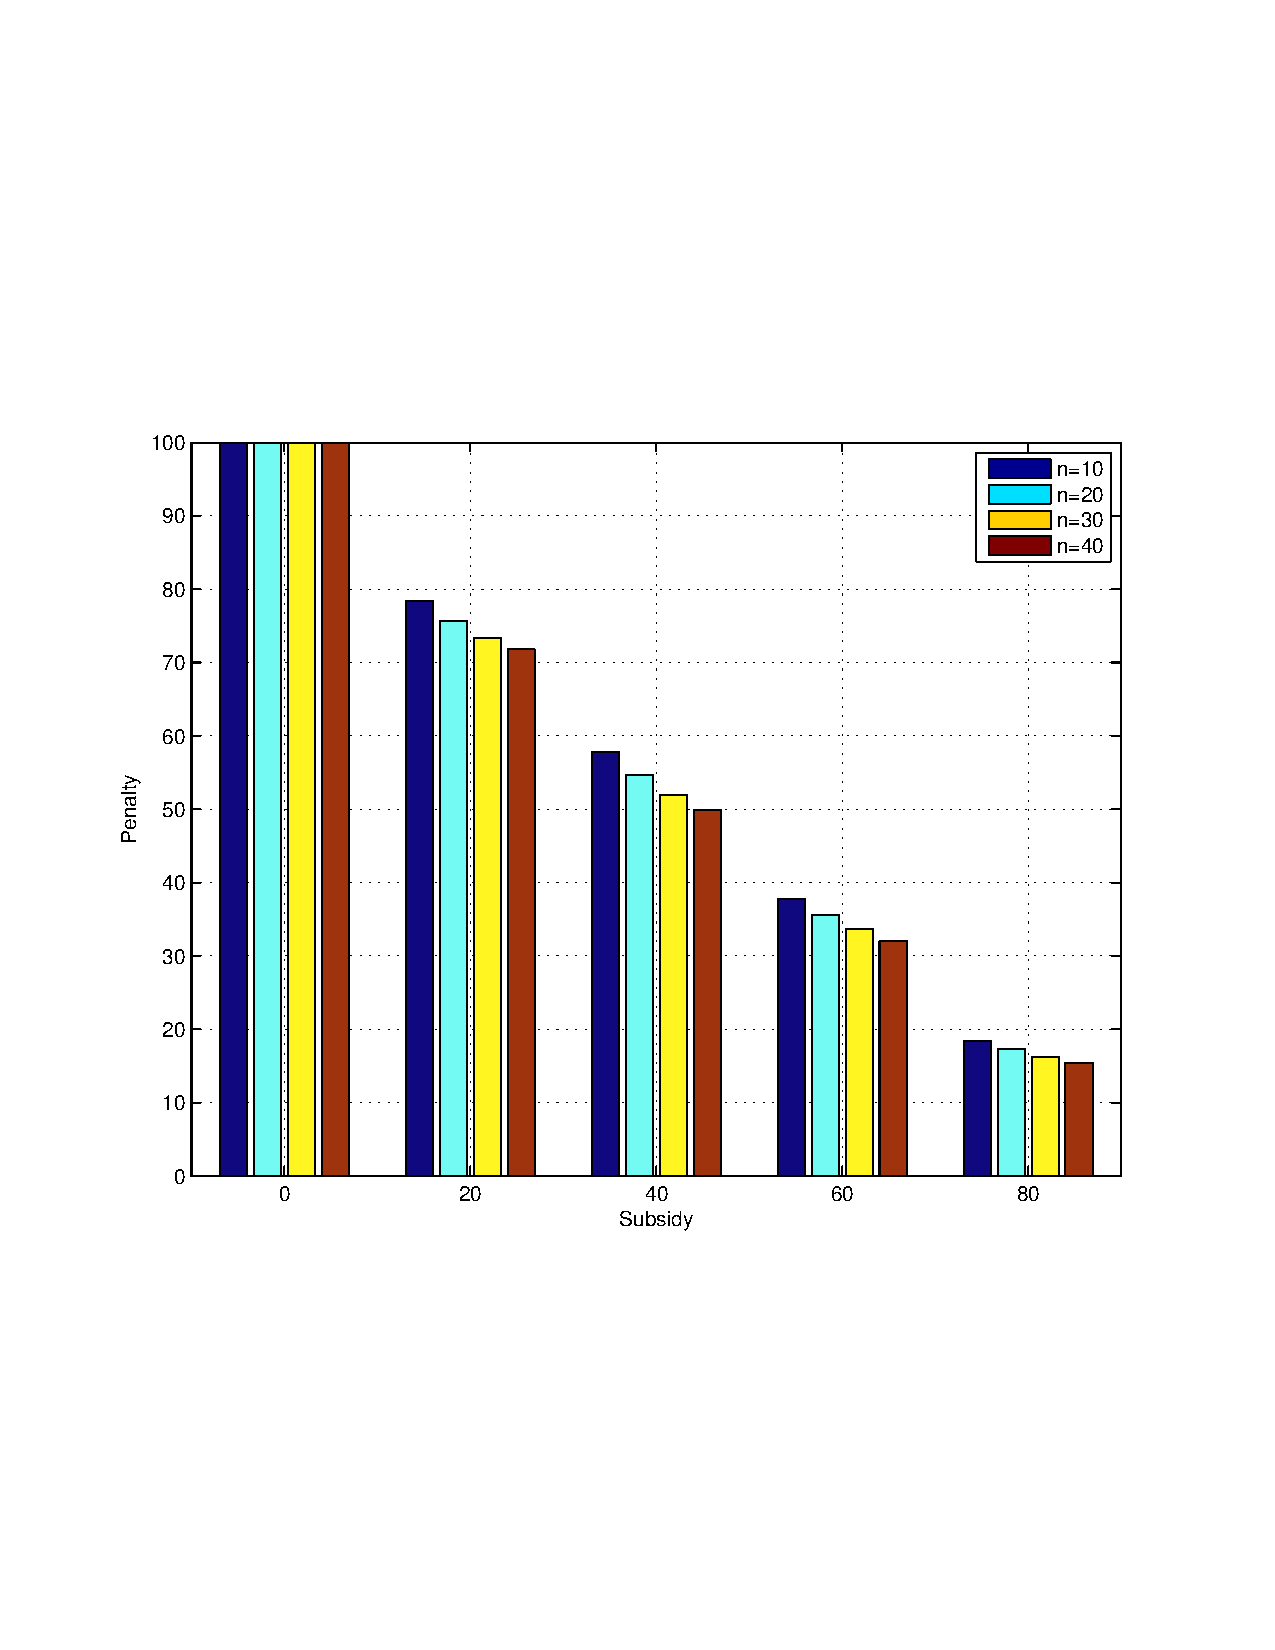
\includegraphics[width=0.55\textwidth]{DifferentSize1.pdf}
\centering
\caption{\label{figure:differentsize}Subsidy efficiency results for different TSP game sizes}
\end{figure}

In addition to the convexity of the Lagrangian SPF as shown in Remark \ref{rem:convex}, the numerical results in Figure \ref{figure:differentsize} imply stronger convexity as the game becomes bigger.
When $n$ is small (e.g. $n = 10$), the subsidy at different levels are almost equally efficient, but when $n$ is large (e.g. $n = 40$), the additional subsidy is much more efficient at the earlier stages than at the later stages.





\section{Conclusion}\label{section:conclusion}
In this paper, we proposed a new LRB heuristic algorithm to compute feasible subsidy--penalty pairs and stabilize grand coalitions in unbalanced cooperative games.
The LRB algorithm is an effective alternative to the existing approaches, such as the CP and LP approaches proposed in \cite{leastcore2018}, especially for IM games with computationally intractable characteristic functions.

We then applied the LRB algorithm to TSP games and computed the Lagrangian subsidized minimum penalty.
By taking good care of the pricing problem, the resulting numerical results confirm that the LRB algorithm is both effective and efficient for TSP games.

The S\&P instrument is a novel idea for stabilizing grand coalitions in cooperative game theory.
However, to apply it to more practical problems, we should have more effective and efficient algorithms to solve feasible subsidy--penalty pairs.
The LRB algorithm is one of such practical algorithms that can lead to interesting results when applied to specific cooperative games.


\section*{Acknowledgement}
This work is partially supported by the National Natural Science Foundation of China [Grant 71701192] and the Fundamental Research Funds for the Central Universities [Grant WK2040160024].


\bibliographystyle{elsarticle-harv}
\bibliography{BibTsp}

\section*{Appendix}
\noindent \textbf{Proof of Theorem \ref{thm:rb}.}\\
The proof is straightforward.
Denote an optimal solution for LP $(\ref{eqn:aSLC})$ as $\big[\beta_r(\ \cdot \ ,\omega),z_r(\omega)\big]$. Now, we consider vector $\big[\bar{\beta}_r(\ \cdot \ ,\omega),z_r(\omega)\big]$, where $\bar{\beta}_r(k,\omega) = \beta_r(k,\omega) - \big(c_u(V)-c(V)\big)/v$, for all $k \in V$. Then, for each $s \in S \setminus V$, we have 
\begin{equation*}
\bar{\beta}_r(s,\omega)  = \beta_r(s,\omega) - \frac{|s|\big[c_u(V)-c(V)\big]}{v} \leq \beta_r(s,\omega) \leq c_l(s)+ z_r(\omega) \leq c(s) + z_r(\omega).
\end{equation*}

Furthermore, since $\bar{\beta}_r(V,\omega) = \beta_r(V,\omega) - \frac{v\big[c_u(V)-c(V)\big]}{v} = c(V)-\omega$, we argue that $\big[ \bar{\beta}_r(\ \cdot \ ,\omega),z_r(\omega) \big]$ is feasible to LP $(\ref{eqn:SLC})$.
Thus, $z_r(\omega)$ is an upper bound of $z(\omega)$.
\qed



\noindent \textbf{Proof of Remark \ref{rem:convex}.}\\
From the strong duality of LP $(\ref{eqn:aSLC})$, we have
\begin{eqnarray}\label{eqn:DualSLC}
\begin{aligned}
z_r(\omega) = \max_{\rho}~ \rho_v \big[ c_u(V)-\omega \big] &- \sum_{s \in S \setminus \{V\}} \rho_s c_l(s)\\
s.t.~~\sum_{s \in S \setminus \{V\}} \rho_s = &1,\\
\sum_{s \in S \setminus \{V\}: k \in s} \rho_s - \rho_v = 0,&~\forall k \in V,\\
\rho_s \geq 0,~\forall s \in& S.
\end{aligned}
\end{eqnarray}
Consequently, $z_r(\omega)$ is the point-wise maximum of a finite set of straight lines, each with a slope of $-\rho_v$.
Thus, $z_r(\omega)$ is a piece-wise linear and convex function  $\omega$.
Moreover, since the slope $-\rho_v$ of each straight line constructing $z_r(\omega)$ is negative ($\rho_v$ is clearly positive), the R-SPF $z_r(\omega)$ must be strictly decreasing in $\omega$.

From the constraints in LP $(\ref{eqn:DualSLC})$, we have 
$$
1 = \sum_{s \in S \setminus \{V\}} \rho_s \leq \sum_{k \in V}\sum_{s \in S \setminus \{V\}: k \in s} \rho_s \leq (v-1)\sum_{s \in S \setminus \{V\}} \rho_s = v-1.
$$
Note that $\sum_{k \in V}\sum_{s \in S \setminus \{V\}: k \in s} \rho_s = v\rho_v$; therefore, we have $1 \leq v\rho_v \leq v-1$, that is $-(v-1)/v\leq -\rho_v \leq -1/v$.
\qed



\noindent \textbf{Proof of Lemma \ref{lemma:equivalentLP}.}\\
Denote an optimal solution of $(\ref{eqn:laSLC})$ as $\big[ \beta_{\lambda}(\ \cdot \ ,\omega), z_{\lambda}(\omega) \big]$. Now, the vector $\big[ \bar{\beta}_{\lambda}(\ \cdot \ ,\omega), z_{\lambda}(\omega) \big]$ with $\big\{\bar{\beta}_{\lambda}(k,\omega) = \beta_{\lambda}(k,\omega) - c_{\lambda1}(k):\forall k \in V\big\}$ is clearly a feasible solution for $(\ref{eqn:l2aSLC})$ since first, for all $s \in S \setminus V$,
\begin{equation*}
\bar{\beta}_{\lambda}(s,\omega) - z_{\lambda}(\omega) = \beta_{\lambda}(s,\omega) - z_{\lambda}(\omega) - c_{\lambda1}(s) \leq c_{\lambda}(s) - c_{\lambda1}(s) = c_{\lambda2}(s),
\end{equation*}
and second,
\begin{equation*}
-\bar{\beta}_{\lambda}(V,\omega) = -\beta_{\lambda}(V,\omega) + c_{\lambda1}(V) \leq -c_{u}(V) + \omega + c_{\lambda1}(V),
\end{equation*}
where $\sum_{k \in s}\bar{\beta}_{\lambda}(k,\omega) = \bar{\beta}_{\lambda}(s,\omega)$ because of the modularity of IM sub-game 1  $(V,c_{\lambda1})$.

Similarly, given the optimal solution $\big[ \beta_{\lambda2}(\ \cdot \ ,\omega), z_{\lambda}(\omega) \big]$ of $(\ref{eqn:l2aSLC})$, we can show that vector $\big[ \bar{\beta}_{\lambda2}(\ \cdot \ ,\omega), z_{\lambda}(\omega) \big]$ with $\big\{\bar{\beta}_{\lambda2}(k,\omega) = \beta_{\lambda2}(k,\omega) + c_{\lambda1}(k):\forall k \in V\big\}$ is feasible for $(\ref{eqn:laSLC})$. Hence, the optimal objective values $z_{\lambda}(\omega)$ of LPs $(\ref{eqn:l2aSLC})$ and $(\ref{eqn:laSLC})$ are the same.
\qed


\noindent \textbf{Proof of Lemma \ref{lemma:up}.}\\
Note that from Theorem \ref{thm:rb}, $z_{\lambda}(\omega)$ is an upper bound of $z(\omega)$ for any given $\omega$.
In addition, from Remark \ref{rem:convex}, the LR-SPF $z_{\lambda}(\omega)$ is convex in $\omega$, implying that $U_{\lambda}(\omega)$ is an upper bound of LR-SPF $z_{\lambda}(\omega)$ and SPF $z(\omega)$.
\qed



\noindent \textbf{Proof of Lemma \ref{lemma:lower}.}\\
The proof is straightforward.
As for the proof of Theorem \ref{thm:rb}, we show that
$$z_{l}(\omega) = \min_{\beta,z} \big\{ z \in \R:\beta(V)=c_\lambda(V)-\omega \mbox{ and } \beta(s) \leq c_u(s)+z, \forall s \in S \setminus V \big\},$$
is a lower bound of $z(\omega)$. 
In addition, we argue that $z_k(\omega) \leq z_{l}(\omega)$, since the latter feasible region is a subset of the former one. 
Therefore, we have $z_k(\omega)\leq z_{l}(\omega) \leq z(\omega)$.
\qed
%%%%%%%%%%%%%%%%%
\end{document}
%%%%%%%%%%%%%%%%%




